\documentclass{article}
\usepackage{algorithm}
\usepackage{algpseudocode}
\usepackage{amsmath,amssymb,amsthm}
\usepackage{graphicx}
\usepackage[margin=1in]{geometry}
\usepackage{fancyhdr}
\usepackage{longtable}
\usepackage{lipsum}
\setlength{\parindent}{0pt}
\setlength{\parskip}{5pt plus 1pt}
\setlength{\headheight}{13.6pt}
\newcommand\question[2]{\vspace{.25in}\hrule\textbf{#1: #2}\hrule\vspace{.10in}}
\renewcommand\part[1]{\vspace{.10in}\textbf{(#1)}}
\newcommand\algo{\vspace{.10in}\textbf{Algorithm: }}
\newcommand\correctness{\vspace{.10in}\textbf{Correctness: }}
\newcommand\runtime{\vspace{.10in}\textbf{Running time: }}
\newcommand\pseudoCode{\vspace{.10in}\textbf{PseudoCode: }}
\newcommand*{\perm}[2]{{}^{#1}\!P_{#2}}
\newcommand*{\comb}[2]{{}^{#1}\!C_{#2}}
%\pagestyle{fancyplain}
%\lhead{\textbf{\NAME\ (\UID)}}
%\chead{\textbf{Hw\HWNUM}}
%\rhead{CS 6150, \today}
\title{CS6150 - Homework/Assignment-3}
\author{Arnab Das(u1014840)}
\usepackage[utf8]{inputenc}
\begin{document}
  \pagenumbering{gobble}
  \maketitle
  \newpage
  \pagenumbering{arabic}
  \newcommand\NAME{ARNAB DAS}
  \newcommand\UID{uxxxxxxx}
  \newcommand\HWNUM{3}

  \question{1}{easy relatives of 3-SAT}
	\part{a} Given a caluse of a 2-CNF formula $x_{1} \vee x_{2}$. Goal is to prove that this clause is logically equivalent to the clause $\bar{x_{1}} \Rightarrow x_{2}$.  The implication clause $\bar{x_{1}} \Rightarrow x_{2}$ means, if $\bar{x_{1}}$ is true, it implies $x_{2}$, else if $\bar{x_{1}}$ is false then the implication doesn't fires and the result is true. Thus, when $\bar{x_{1}}$ is false(or $x_{1}$ is true), the clause is always true regardless of $x_{2}$. When $\bar{x_{1}}$ is true, it implies the clause is determined by the result of $x_{2}$, that is if $x_{2}$ is true, then the result is true, and if $x_{2}$ is false, the result is false. Thus, if we make the truth table of $\bar{x_{1}} \Rightarrow x_{2}$, the table will look as below: \newline
\begin{table}[ht]
  \caption{Truth Table of $\bar{x_{1}} \Rightarrow x_{2}$}
  \centering
  \begin{tabular}{c c c }
  \hline\hline
  $\bar{x_{1}}$ & $x_{2}$ & $\bar{x_{1}} \Rightarrow x_{2}$ \\[0.5ex]
  \hline
  0 & 0 & 1 \\
  0 & 1 & 1 \\
  1 & 0 & 0 \\
  1 & 1 & 1 \\ [0.5ex]
  \end{tabular}
  \label{table:nonlin}
  \end{table}	  

Below is the truth table of $x_{1} \vee x_{2}$ \newline
\begin{table}[ht]
  \caption{Truth Table of $x_{1} \vee x_{2}$}
  \centering
  \begin{tabular}{c c c }
  \hline\hline
  $\bar{x_{1}}$ & $x_{2}$ & ${x_{1}} \vee x_{2}$ \\[0.5ex]
  \hline
  0 & 0 & 1 \\
  0 & 1 & 1 \\
  1 & 0 & 0 \\
  1 & 1 & 1 \\ [0.5ex]
  \end{tabular}
  \label{table:nonlin}
  \end{table}	 

  The truth tables of table-1 and table-2 are exactly the same thus implying that the clause $x_{1} \vee x_{2}$ is equivalent to $\bar{x_{1}} \Rightarrow x_{2}$. \newline

  \part{b} Suppose we have a 2-CNF formula, comprising of m-clauses. It is unsatisfiable if their exists a clause $(x_{i} \vee x_{j})$, such that we have combination like \newline
\begin{equation}
   (x_{i} \vee x_{j})\wedge \bar{x_{i}} \wedge \bar{x_{j}}
\end{equation}
This is unsatisfiable because, $\bar{x_{i}}$ and $\bar{x_{j}}$  will require an assignment of $x_{i}=0$ and $x_{j} = 0$ for them to be true. However, this assignment will result in $(x_{i} \vee x_{j})$ to be false and hence unsatisfiable. This above combination of clauses can be further decomposed into the following pieces for ease of analysis. \newline
	\hspace*{0.5cm} (1). $\bar{x_{i}}$ in a 2-cnf form will be generated if there exists a path such that $(\bar{x_{i}} \vee \bar{x_{i}})$ equivalent to $(x_{i} \Rightarrow \bar{x_{i}})$ is present. \newline
      \hspace*{0.5cm} (2).  $\bar{x_{j}}$ in a 2-cnf form will be generated if there exists a path such that $(\bar{x_{j}} \vee \bar{x_{j}})$ equivalent to $(x_{j} \Rightarrow \bar{x_{j}})$ is present. \newline
	\hspace*{0.5cm} (3). Also, $(x_{i} \vee x_{j})$ can be written in either form of $(\bar{x_{i}} \Rightarrow x_{j})$ and $(\bar{x_{j}} \Rightarrow x_{i})$ \newline

If we consider a directed graph, where each literal is a node(thus for n variables there will be 2n literals) and the clause $(a \Rightarrow b)$ indicates an edge from node 'a' to node 'b', then the above 4 clauses will result in the following connectivity.\newline

  \begin{figure}[h!]
   \centering
  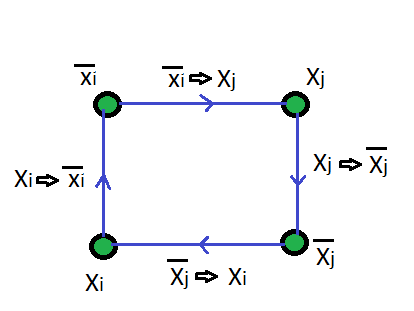
\includegraphics[width=5cm, height=5cm]{Prob1b}
  \caption{The cycle representation for unsatisfiability}
  \end{figure}

 As the figure suggests, the above formation of clauses results in a cycle. Note that the absence of any of the above caluses will result in a valid assignment, which from the perspective of the graph means that the cycle breaks resulting in a valid assignment. Existence of the cycle implies that there is a path from $x_{i}$ to $\bar{x_{i}}$ and from $\bar{x_{i}}$ to $x_{i}$, which essentially makes the 2-CNF formula unsatisfiable. (Proved)
Thus, satisfiability of a 2-CNF formula requires searching for the existence of such a cycle which can be easily found by using a Breath first search(BFS) which is of $O(|E|+|V|)$, where $|E| and |V|$ are the cardinality of the edges and vertices of the graph respectively. Thus, finding satisfiability of a 2-CNF formula is polynomial time.\newline

\part{c} A problem for 2-or-more  3SAT is defined as follows: Given a 3-CNF formula, $\phi$, an assignment is said to 2-or-more satisfy a clause iff atleast two of the literals in that clause are true for that assignment. \textbf {Goal:} To prove that there exists an assignment that 2-or-more 3SAT has a polynomial time algorithm. \newline

\textbf{Proof:} \newline
\textbf{Claim:} A 3-CNF clause, say, $(x_{i} \vee x_{j} \vee x_{k})$ , is 2-or-more satisfiable if the CNF breakdown of its $^3C_{2}$ combinations are satisfiable, that is, we can rewrite $(x_{i} \vee x_{j} \vee x_{k})$ as \newline
\begin{equation}
	(x_{i} \vee x_{j} \vee x_{k}) = (x_{i} \vee x_{j}) \wedge (x_{j} \vee x_{k}) \wedge (x_{k} \vee x_{i})
\end{equation}
This claim can be easily verified by constructing the truth tables of the lhs and the rhs of the equation as given below, \newline
\begin{table}[ht]
  \caption{Truth Table of 2-or-more($x_{i} \vee x_{j} \vee x_{k}$)}
  \centering
  \begin{tabular}{c c c c}
  \hline\hline
   $x_{i}$ & $x_{j}$ & $x_{k}$ & 2-or-more($x_{i} \vee x_{j} \vee x_{k}$) \\[0.5ex]
  \hline
  0 & 0 & 0 & 0 \\
  0 & 0 & 1 & 0 \\
  0 & 1 & 0 & 0 \\
  0 & 1 & 1 & 1 \\
  1 & 0 & 0 & 1 \\
  1 & 0 & 1 & 1 \\
  1 & 1 & 0 & 1 \\
  1 & 1 & 1 & 1 \\
  \end{tabular}
  \label{table:nonlin}
  \end{table}	  

\begin{table}[ht]
  \caption{Truth Table of $(x_{i} \vee x_{j}) \wedge (x_{j} \vee x_{k}) \wedge (x_{k} \vee x_{i})$}
  \centering
  \begin{tabular}{c c c c c c c}
  \hline\hline
  $x_{i}$ &  $x_{j}$ & $x_{k}$ & $(x_{i} \vee x_{j})$ & $(x_{j} \vee x_{k})$ & $(x_{k} \vee x_{i})$ & $(x_{i} \vee x_{j}) \wedge (x_{j} \vee x_{k}) \wedge (x_{k} \vee x_{i})$  \\[0.5ex]
  \hline
  0 & 0 & 0 & 0 & 0 & 0 & 0 \\
  0 & 0 & 1 & 0 & 1 & 1 & 0 \\
  0 & 1 & 0 & 1 & 1 & 0 & 0 \\
  0 & 1 & 1 & 1 & 1 & 1 & 1 \\
  1 & 0 & 0 & 1 & 1 & 1 & 1 \\
  1 & 0 & 1 & 1 & 1 & 1 & 1 \\
  1 & 1 & 0 & 1 & 1 & 1 & 1 \\
  1 & 1 & 1 & 1 & 1 & 1 & 1 \\ [0.5ex]
  \end{tabular}
  \label{table:nonlin}
  \end{table}

As the truth tables of Table-3 and Table-4 suggest the equivalence of equation-2, we will use this claim to breakdown the clauses. Thus each 3-CNF clause is broken down to 3 2-CNF clauses. For m clauses of the original formula, $\phi$, there will be 3m number of 2-CNF clauses, which is a \textbf {polynomial} time breakdown. Next, we just need to solve a 2-CNF $\phi$ of 3m clauses, and we have already proved in the last question(1b) that such a formula has a \textbf {polynomial} time algorithm. \newline
Thus the overall complexity of the algorithm comprises of firstly, a breakdown from 3-CNF to 2-CNF which is \textbf {polynomial} time, and secondly, solving a 2-CNF which is again \textbf {polynomial} time. Thus we caan conclude that 2-or-more 3SAT has a polynomial time algorithm. \newline

\question{2}{Decision vs Search}
Given an undirected graph, G=(V,E), a parameter k and an Oracle that answers Yes/No when a query is sent to it in the form of two inputs, the graph G and the parameter k. It answers Yes if G has an independent set of size k and No otherwise. \newline
\textbf {Goal:} To prove that there exists an algorithm that can find an independent set of size k, if one exists, by making polynomial amount of calls to the Oracle and a polynomial amount of computations of its own. 

\algo \newline
	\textbf {findIndSet}(G,k) \{ \newline
	\hspace*{0.5cm} ans = Oracle(G,k) \newline
	\hspace*{0.5cm} \textbf {if}(ans==No) return NULL \newline
	\hspace*{0.5cm} \textbf {else} \{ \newline
	\hspace*{1cm}		i = $\phi$ ; IndSet = \{\}; \newline
	\hspace*{1cm}		\textbf {while} ( k $>$ 0) \{; \newline
	\hspace*{1.5cm}			G = G - i ; \newline
	\hspace*{1.5cm}			i  = SelectNode(G) ; \newline
	\hspace*{1.5cm}			$G^\prime$ = StripG(G, i) ; \newline
	\hspace*{1.5cm}			ans = Oracle($G^\prime$, k-1); \newline
	\hspace*{1.5cm}			\textbf {if}(ans==Yes) \{ \newline
	\hspace*{2cm}				IndSet = IndSet $\cup$ i ; \newline
	\hspace*{2cm}				G = $G^\prime$ ; \newline
	\hspace*{2cm}				k = k - 1 ;  \newline
	\hspace*{1.5cm}			\} \newline
	\hspace*{1cm}		\} \newline
	\hspace*{0.5cm}	\} \newline
	\} \newline







\end{document} 
